\documentclass[11pt, oneside]{article}
\usepackage[letterpaper, margin=2cm]{geometry}
\usepackage{MATH566}
%\usepackage{sagetex}

\begin{document}
\noindent \textbf{\Large{Caleb Logemann \\
MATH 566 Discrete Optimization\\
Homework 2
}}

%\lstinputlisting[language=Matlab]{H01_23.m}
\begin{enumerate}
    \item % #1 Done
        \begin{enumerate}
            \item[(a)]
                Give an example of bounded convex sets $C$ and $D$ in $\RR^d$,
                where $C \cap D = \varnothing$, but there is no hyperplane
                stricly seperating $C$ and $D$.
                That is find $a \in \RR^d$ and $b \in \RR$, such that
                \[
                    \v{a}^T\v{c} > b, \forall \v{c} \in C \quad \text{and} \quad \v{a}^T\v{d} < b, \forall \v{d} \in D
                \]

                Let $C = \set{\br{x, y}^T | -1 < x < 0, 0 < y < 1} \cup \set{\br{0, 0}^T}$
                and let $D = \set{\p{x, y} | 0 < x < 1, 0 < y < 1} \cup \set{\br{0, 1}^T}$.
                In this case $C$ and $D$ are bounded convex sets and $C \cap D = \varnothing$.
                Let $\v{a} = \br{-1, 0}^T$ and $b = 0$, then for $\v{c} \in C$,
                $\v{a}^T \v{c} \ge 0$ and if $\v{c} = \br{0, 0}$, then $\v{a}^T \v{c} = 0$.
                Also for $\v{d} \in D$, $\v{a}^T \v{d} \le 0$ and for $\v{d} = \br{0, 1}^T$,
                $\v{a}^T \v{d} = 0$.
                Therefore there is no hyperplane strictly seperating $C$ and $D$.

                A plot of these regions is shown below
                \begin{center}
                    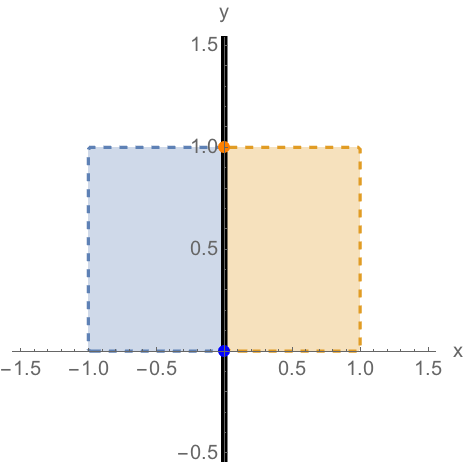
\includegraphics[scale=.4]{Figures/02_2.png}
                \end{center}

            \item[(b)]
                Give an example of closed convex sets $C$ and $D$ that cannot
                be strictly seperated.

                Let $C = \set{\br{x, y}^T | xy >= 1, x >= 0}$, and let
                $D = \set{\br{x, y}^T | x \le 0}$.
                In this case $C$ and $D$ are closed convex sets and
                $C \cap D = \varnothing$.
                Then it is required that $\v{a} = \br{1, 0}^T$ and $b = 0$.
                For $\v{c} \in C$, $\v{a}^T \v{c} > 0$.
                Also $\v{d} \in D$, $\v{a}^T \v{d} \le 0$.
                Therefore there is no hyperplane strictly seperating $C$ and $D$.

                A plot of these regions is shown below
                \begin{center}
                    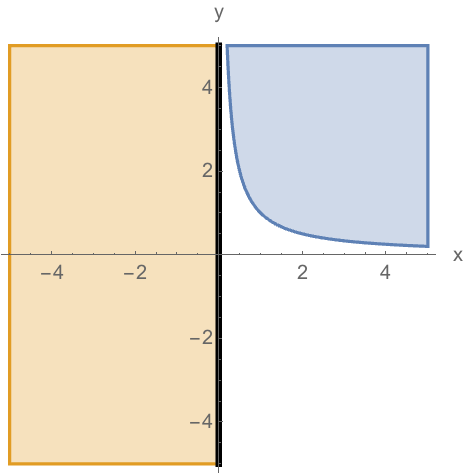
\includegraphics[scale=.4]{Figures/02_1.png}
                \end{center}
        \end{enumerate}

    \item % #2 Done
        Dualize your diet problem.
        Take the data from your diet problem from HW1, create the dual of the
        program, and solve it.
        Your answer should contain the solution of the dual and the
        interpretation of the results of the dual.

        The original diet problem can be written as
        \[
            \begin{array}{ll@{}ll}
                \min* & \v{c}^T \v{x} \\
                \text{s.t.} & A\v{x} \ge \v{b} \\
                            & \v{x} \ge \v{0}
            \end{array}
        \]
        where
        \begin{align*}
            A^T =
            \begin{bmatrix}
                125 & 35 & 0 &  0 & 0.275 \\ % 1
                190 &  7 & 2 &  7 & 0.130 \\ % 2
                110 & 27 & 1 &  0 &     0 \\ % 3
                 50 & 13 & 0 &  0 &     0 \\ % 4
                190 & 27 & 1 &  4 & 0.360 \\ % 5
                100 & 18 & 1 &  2 &  0.06 \\ % 6
                 60 &  9 & 2 &  2 &   0.2 \\ % 7
                 20 &  4 & 2 &  1 &  0.38 \\ % 8
                 70 & 12 & 3 &  4 &  0.37 \\ % 9
                 60 & 25 & 4 &  2 & 0.105 \\ % 10
                120 &  2 & 0 &  1 & 0.025 \\ % 11
                140 & 24 & 1 &  4 &  0.44 \\ % 12
                 80 &  1 & 0 &  8 &  0.69 \\ % 13
                 60 &  0 & 0 & 11 &  0.52 \\ % 14
                150 & 25 & 1 &  4 & 0.025    % 15
            \end{bmatrix}
            \v{b} =
            \begin{bmatrix}
                2779 \\
                 383 \\
                  38 \\
                  60 \\
                 1.5
            \end{bmatrix}
            \v{c} =
            \begin{bmatrix}
                0.75 \\ % 1
                0.13 \\ % 2
                0.34 \\ % 3
                0.13 \\ % 4
                0.48 \\ % 5
                0.17 \\ % 6
                0.21 \\ % 7
                0.21 \\ % 8
                0.21 \\ % 9
                0.25 \\ % 10
                0.42 \\ % 11
                0.26 \\ % 12
                0.50 \\ % 13
                1.15 \\ % 14
                0.29    % 15
            \end{bmatrix}
        \end{align*}
        and $\v{x}$ is the number of servings of each type of food.

        The dual of the diet program can be written as follows
        \[
            \begin{array}{ll@{}ll}
                \min* & \v{b}^T \v{y} \\
                \text{s.t.} & A^T\v{y} \ge \v{c} \\
                            & \v{y} \ge \v{0}
            \end{array}
        \]

        The dual of the program can be written in Sage as follows.
        \lstinputlisting[language=Sage]{02_2.sage}
        \begin{verbatim}
            Objective Value: 3.95434986206
            y_1 = 0.000327791491215
            y_2 = 0.00715914040947
            y_3 = 0.00299840278786
            y_4 = 0.0
            y_5 = 0.08929867867
        \end{verbatim}

        The objective solution is \$3.95 a day which is identical to the
        solution found in homework 1.
        The solution values are \$0.0003277 per calorie, \$0.007159 per carb,
        \$0.002998 per gram of fiber, \$0 per gram of protein, and
        \$0.089298 per gram of sodium.

    \item % #3 Done
        A paper mill manufactures rolls of paper of a standard width, 3 meters.
        But customers want to buy rolls of shorter width, and the mill has to
        cut such rolls from the 3m rolls.
        Let us consider an order of
        \begin{itemize}
            \item 97 rolls of width 135 cm,
            \item 610 rolls of width 108 cm,
            \item 395 rolls of width 93 cm, and
            \item 211 rolls of width 42 cm.
        \end{itemize}
        What is the smallest number of 3m rolls that have to be cut in order to
        satisfy this order?

        First we must enumerate all of the different ways that a 3m roll can be
        cut up into these lengths.
        \begin{enumerate}
            \item $c_1 = 2 \times 135$
            \item $c_2 = 135 + 108 + 42$
            \item $c_3 = 135 + 93 + 42$
            \item $c_4 = 135 + 3 \times 42$
            \item $c_5 = 2 \times 108 + 2 \times 42$
            \item $c_6 = 108 + 2 \times 93$
            \item $c_7 = 108 + 93 + 2 \times 42$
            \item $c_8 = 108 + 4 \times 42$
            \item $c_9 = 3 \times 93$.
            \item $c_{10} = 2 \times 93 + 2 \times 42$
            \item $c_{11} = 93 + 4 \times 42$
            \item $c_{12} = 7 \times 42$
        \end{enumerate}
        Any other cuts leave excess paper that could be used for the order so
        won't be necessary.

        Then we can create the integer linear program.
        \[
            \begin{array}{ll@{}ll}
                \min* & \displaystyle\sum{i = 1}{12}{c_i} & & \\
                \text{s.t.} & 2c_1 + c_2 + c_3 + c_4 \ge 97 \\
                & c_2 + 2c_5 + c_6 + c_7 + c_8 \ge 610 \\
                & c_3 + 2 c_6 + c_7 + 3c_9 + 2c_{10} + c_{11} \ge 395 \\
                & c_2 + c_3 + 3c_4 + 2c_5 + 2c_7 + 4c_8 + 2c_{10} + 4c_{11} + 7c_{12} \ge 211 \\
                & c_i \ge 0 \quad 1 \le i \le 12 \\
                & c_i \in \ZZ \quad 1 \le i \le 12
            \end{array}
        \]

        This integer linear program can be written in Sage as follows
        \lstinputlisting[language=Sage]{02_3.sage}

        The solution given by Sage is
        \begin{verbatim}
            Objective Value: 453.0
            c_1 = 49
            c_2 = 0
            c_3 = 0
            c_4 = 0
            c_5 = 206
            c_6 = 198
            c_7 = 0
            c_8 = 0
            c_9 = 0
            c_10 = 0
            c_11 = 0
            c_12 = 0
        \end{verbatim}

        This means that 453 3 m rolls are needed in order to fill this order.
        Of the 453 rolls, 49 should be cut into two 135 cm rolls, 206 shold be
        cut into two 108 cm rolls and two 42 cm rolls, and the remaining 198
        rolls should be cut into a 108 cm roll and two 93 cm rolls
\end{enumerate}
\end{document}
